\section{February 28}
\subsection{Rectangular Wave Guide}
Now we will consider the special case where the cross section of our wave guide happens to be a perfect
rectangle. We will consider TE modes, so \( E_z = 0 \). So our objective is to solve for \( B_z \), using the
wave equation. The differential equation we want to solve is 
\[
	\left( \partial_x^2 + \partial_y^2 + \left( \frac{\omega}{c} \right)^2 - k^2 \right)B_z = 0
\]
This equation is actually solved in a very similar way to the infinite square well in quantum mechanics. We
will assume separable solutions of the form \( B_z(x,y) = X(x) Y(y) \). Then, the wave equation becomes:  
\[
	Y \partial_x^2 X + X \partial_y^2 Y + \left( \frac{\omega}{c} \right)^2 XY - k^2 XY = 0
\]
Dividing both sides by \( XY \), we get:
\[
	\frac{1}{X}\partial_x^2 X + \frac{1}{Y}\partial_y^2 Y + \left( \frac{\omega^2}{c^2} - k^2 \right) = 0
\]
Notice here that the first term only has \( x \) dependence, and the second term only has \( y \) dependence.
Therefore, for this to equal zero at all times, then we require that both these values must be constants.
Therefore, we will call:
\[
	\frac{1}{X}\partial_x^2 X = -k_x^2 \quad \frac{1}{Y}\partial_y^2 Y = -k_y^2
\]
We choose \( k_x \) and \( k_y \) such that \( k_X^2 + k_y^2 + k^2 = \left( \frac{\omega}{c} \right)^2 \).
The two separate differential equations now admit solutions of the form:
\begin{align*}
	X(x) &= A \sin (k_x x) + B \cos (k_x x) \\ 
	Y(y) &= A \sin (k_y y) + B \cos (k_y y)
\end{align*}
Now, we impose the boundary conditions: \( \tilde E_{\parallel} = 0 \) and \( \tilde B_{\perp} =
0 \). Since 
\[
	B_x = \frac{i}{\left( \frac{\omega}{c} \right)^2 - k^2}\left[ k \partial_x B_z -
	\frac{\omega}{c^2}\partial_y E_z \right]
\]
and \( E_z = 0 \) because of TE waves, then we have \( \partial_x B_z\eval_{x = 0, a} = 0 \) as a result. The
boundary conditions come down to \( \partial_x X \eval_{x = 0, a} = 0 \), which gives the condition:
\[
	k_xa = m \pi \implies k_x = \frac{m\pi}{a}
\]
Similarly, we can get \( k_y = \frac{n\pi}{b} \). 

\subsection{Cutoff Frequency}
With the differential equation solved, the equation for \( \mathbf{B} \) is now: 
\[
	\tilde B(x, y) = B_0 \cos\left( \frac{m \pi x}{a} \right) \cos\left( \frac{n \pi y}{b} \right)
\]
We also have the constraint \( k_x^2 + k_y^2 + k^2 = \left( \frac{\omega}{c} \right)^2 \), so this means:
\[
	k = \sqrt{\left( \frac{\omega}{c} \right)^2 - \left( \frac{m\pi}{a} \right)^2 - \left( \frac{n\pi}{b}
	\right)^2}
\]
This equation has an interesting consequence: if \( \left( \frac{\omega}{c} \right)^2 < \left( \frac{m\pi}{a}
\right)^2 + \left( \frac{n\pi}{b} \right)^2 \), then \( k \) becomes imaginary, and this eventually means
that the wave now decays over time, and you won't get a propagating wave. So this means that there is a
minimum frequency below which you can't get a propagating wave, which is given by the cutoff frequency
\[
	\omega_{mn} = c \pi \sqrt{\left( \frac{m}{a} \right)^2 + \left( \frac{n}{b} \right)^2}
\]
\subsection{Phase Velocity}
In a wave guide, it is possible for the phase velocity to exceed the group velocity. Consider a wave with
angular velocity \( k = \frac{1}{c}\sqrt{\omega^2 - \omega_{mn}^2} \). Then, the phase speed in the \( z \)
direction is given by:
\[
	v_\text{phase} = \frac{\omega}{k} = c \cdot \frac{\omega}{\sqrt{\omega^2 - \omega_{mn}^2}} > c
\]
How is this allowed behavior? The reason is because it is impossible to encode information in the phase of a
wave, and instead we encode it in the frequency, which travels at the \textit{group velocity}:
\[
	v_\text{group} = \dv{\omega}{k} = \left( \dv{k}{\omega} \right)^{-1} = c \cdot \frac{\sqrt{\omega^2 -
	\omega_{mn}^2}}{\omega} < c
\]
which is less than \( c \), so there is no violation of causality here. There is also a nice physical picture
for this result: consider a wave propagating through the wave guide, and here we will explicitly draw out the
wavefront:
\begin{center}
	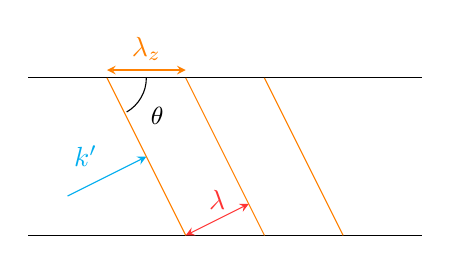
\begin{tikzpicture}
		\draw (0, 1) -- (5, 1);
		\draw (0, -1) -- (5, -1);
		\foreach \x in {1, 2, 3} {
			\draw[color=orange] (\x, 1) -- (\x+1, -1);
		}
		\draw[stealth-stealth, orange] (1, 1.1) -- node[midway, above] {\( \lambda_z \)} (2, 1.1);
		\draw[color=cyan, -stealth] (0.5, -0.5) -- node[midway, above left] {\( k' \)} (1.5, 0);
		\draw (1.5, 1) arc [radius = 0.5, start angle = 0, delta angle = -60] node[midway, below right]
			{\small \( \theta \)};
		\draw[color=red!80!white, stealth-stealth] (2, -1) -- node[midway, above] {\( \lambda \)} (2.8, -0.6); 
	\end{tikzpicture}
\end{center}
The actual wavelength \( \lambda \) is calculated as the perpendicular distance between two wavefronts, so
using this definition we see that there's a pretty simple equation for \( \lambda_z \):
\[
	\lambda_z = \frac{\lambda}{\cos \theta}
\]
And because we need to form standing waves, we have \( |k'| \cos \theta = \frac{\lambda}{k} \), so:
\[
	\cos \theta = \frac{k}{|k'|} = \sqrt{1 - \left( \frac{\omega_{mn}}{\omega} \right)^2}
\]
Now, the group velocity is given by how fast it travels in the \( z \) direction, so \( v_g = c \cos \theta
\), therefore we have:
\[
	v_g = c \sqrt{1 - \left( \frac{\omega_{mn}}{\omega} \right)^2}
\]
and we get the same result that the group velocity is less than \( c \). 

       



